\documentclass{beamer}

%\usetheme[framenumber,totalframenumber]{UniversiteitGent}
%\usetheme[faculty=di,framenumber,totalframenumber]{UniversiteitGent}
%\usetheme[faculty=we,usecolors,framenumber,totalframenumber]{UniversiteitGent}
%\usetheme[language=english,framenumber,totalframenumber]{AlleghenyCollege}
\usetheme{AnnArbor}
\usecolortheme{dove}

\title{CMPSC 390 \\ Ethereum and Smart Contracts. Altcoins.}
\author{Janyl Jumadinova \\ $ $ \\ Credit: Authors of ``Mastering Bitcoin" and ``Bitcoin and Cryptocurrency Technologies"}
\date{February 2, 2021}

\long\def\omitit#1{}

\usepackage{hyperref}
\hypersetup{
    colorlinks=true,
    linkcolor=blue,
    filecolor=magenta,      
    urlcolor=cyan,
}

\usepackage{color, soul}

\begin{document}

\begin{frame}
  \titlepage
\end{frame}

%%%%%%%%%%%% Slide %%%%%%%%%%%%%%%%%%%%%%%%%%%%%%%%%%%%%%%%%%%%%%%%%%%
\begin{frame}
  \frametitle{Transferable Benefits of Bitcoin }
	\begin{itemize}
		\item \textcolor{brown}{Pseudonymous}, cryptographic identities allow  for accountability. \pause
		\item \textcolor{brown}{Democratic} decisions made through consensus  protocol that doesn't require trust. \pause
		\item \textcolor{brown}{Immutable} ledger of truth. \pause
		\item \textcolor{brown}{Uncensorable}, cannot be controlled by any one party. \pause
		\item \textcolor{brown}{Distributed}: no central point of failure.

	\end{itemize}
\end{frame}
%%%%%%%%%%%% Slide %%%%%%%%%%%%%%%%%%%%%%%%%%%%%%%%%%%%%%%%%%%%%%%%%%%
\begin{frame}
  \frametitle{Smart Contracts}
  Code that \textbf{facilitates}, \textbf{verifies}, or \textbf{enforces} the negotiation or execution of a digital contract.

 	\centering
	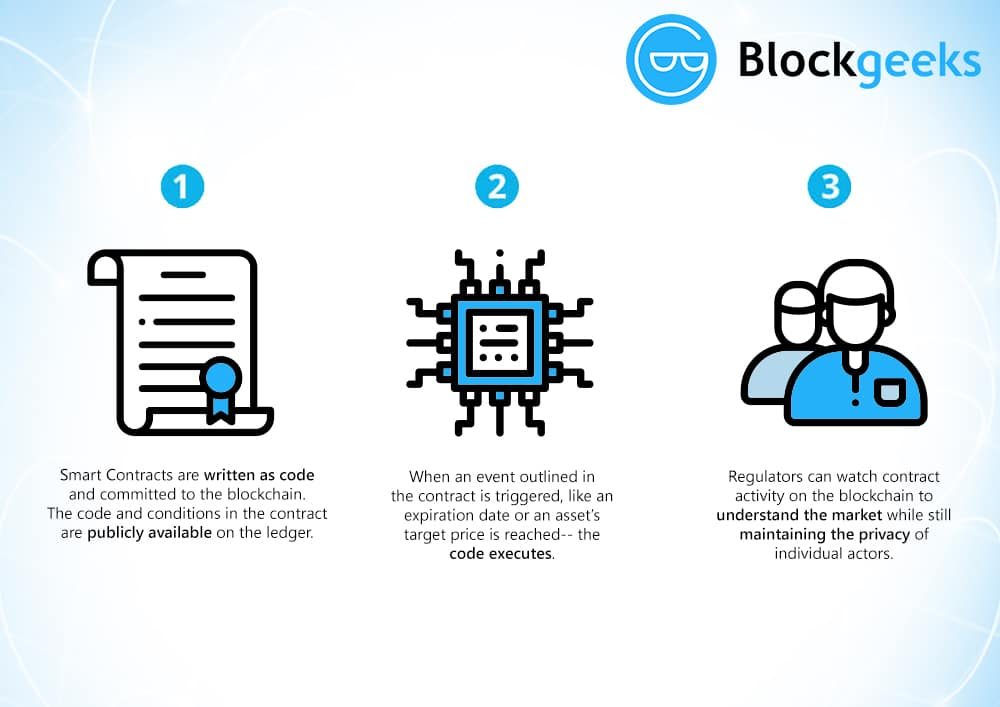
\includegraphics[scale=0.28]{smart.jpg}
\end{frame}
%%%%%%%%%%%% Slide %%%%%%%%%%%%%%%%%%%%%%%%%%%%%%%%%%%%%%%%%%%%%%%%%%%
\begin{frame}
  \frametitle{Ethereum}
	\url{https://ethereum.org}
	\pause
	\begin{block}{\emph{Ethereum is a decentralized platform designed to run smart contracts}:}
	\begin{itemize}
		\item Distributed computer to execute code. \pause
		\item Account-based blockchain. \pause
		\item Transactions == state transaction function. \pause
		\item Ethereum's  native asset is called \textcolor{brown}{ether}: 
			-- Basis of value in the Ethereum ecosystem.
	\end{itemize}
	\end{block}
\end{frame}
%%%%%%%%%%%% Slide %%%%%%%%%%%%%%%%%%%%%%%%%%%%%%%%%%%%%%%%%%%%%%%%%%%
\begin{frame}
  \frametitle{Ethereum}
  	\begin{itemize}
  		\item \textbf{Block creation time}: $~13 sec$ (Ethereum) vs $~10 min$ (Bitcoin)
  		\item Ethereum price:
  	\end{itemize}
 	\centering
	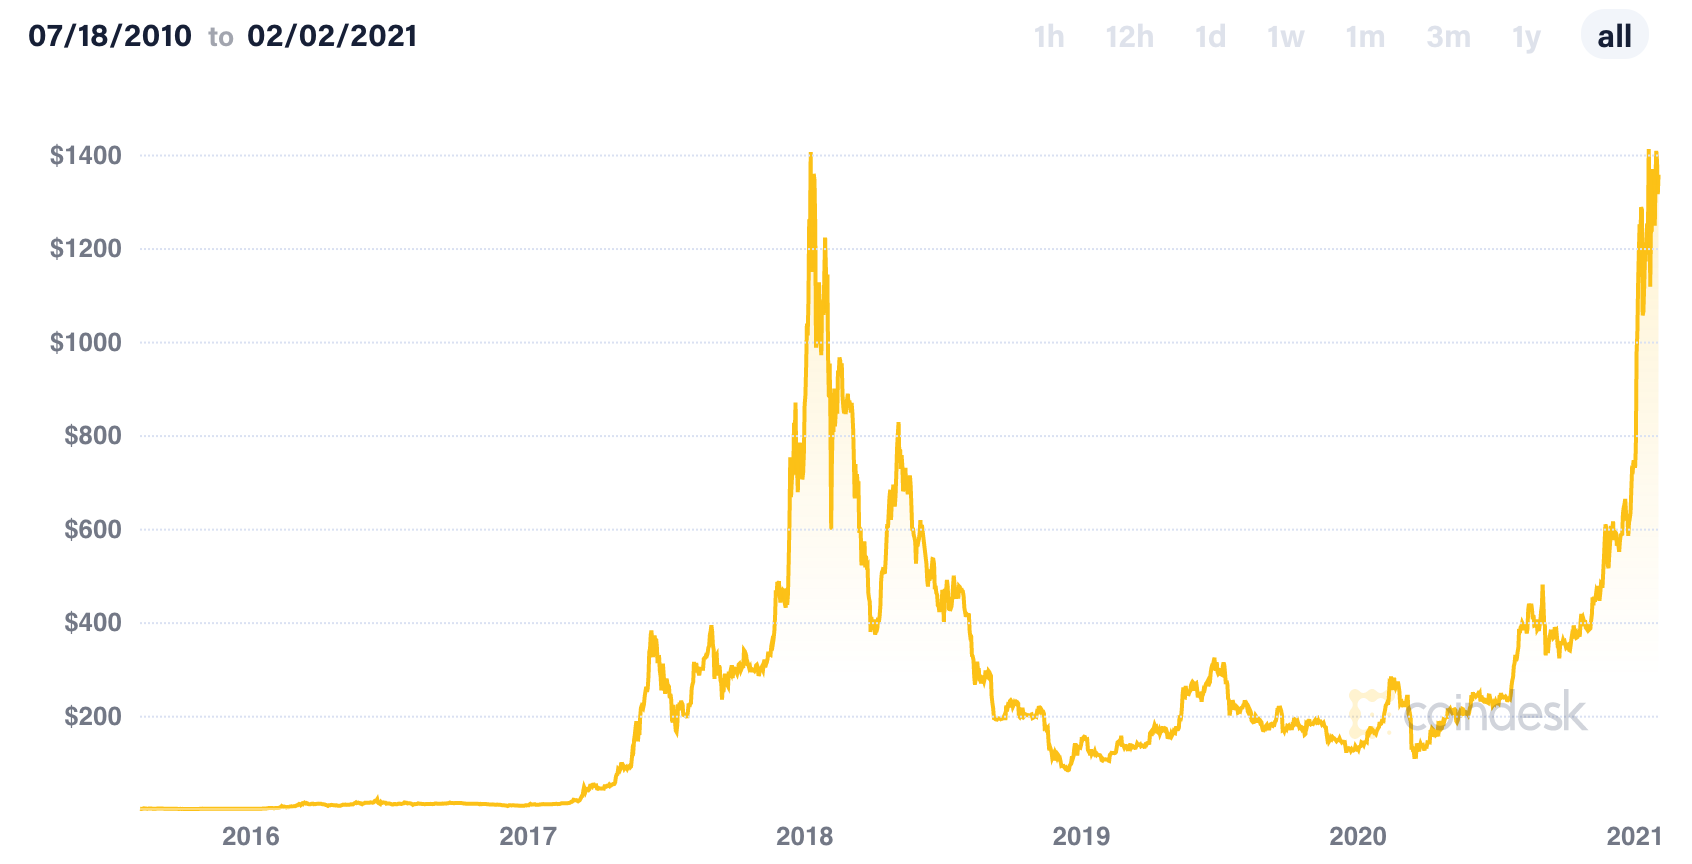
\includegraphics[scale=0.32]{etherium}
\end{frame}

%%%%%%%%%%%% Slide %%%%%%%%%%%%%%%%%%%%%%%%%%%%%%%%%%%%%%%%%%%%%%%%%%%
\begin{frame}
  \frametitle{Bitcoin vs. Ethereum}
 	\centering
	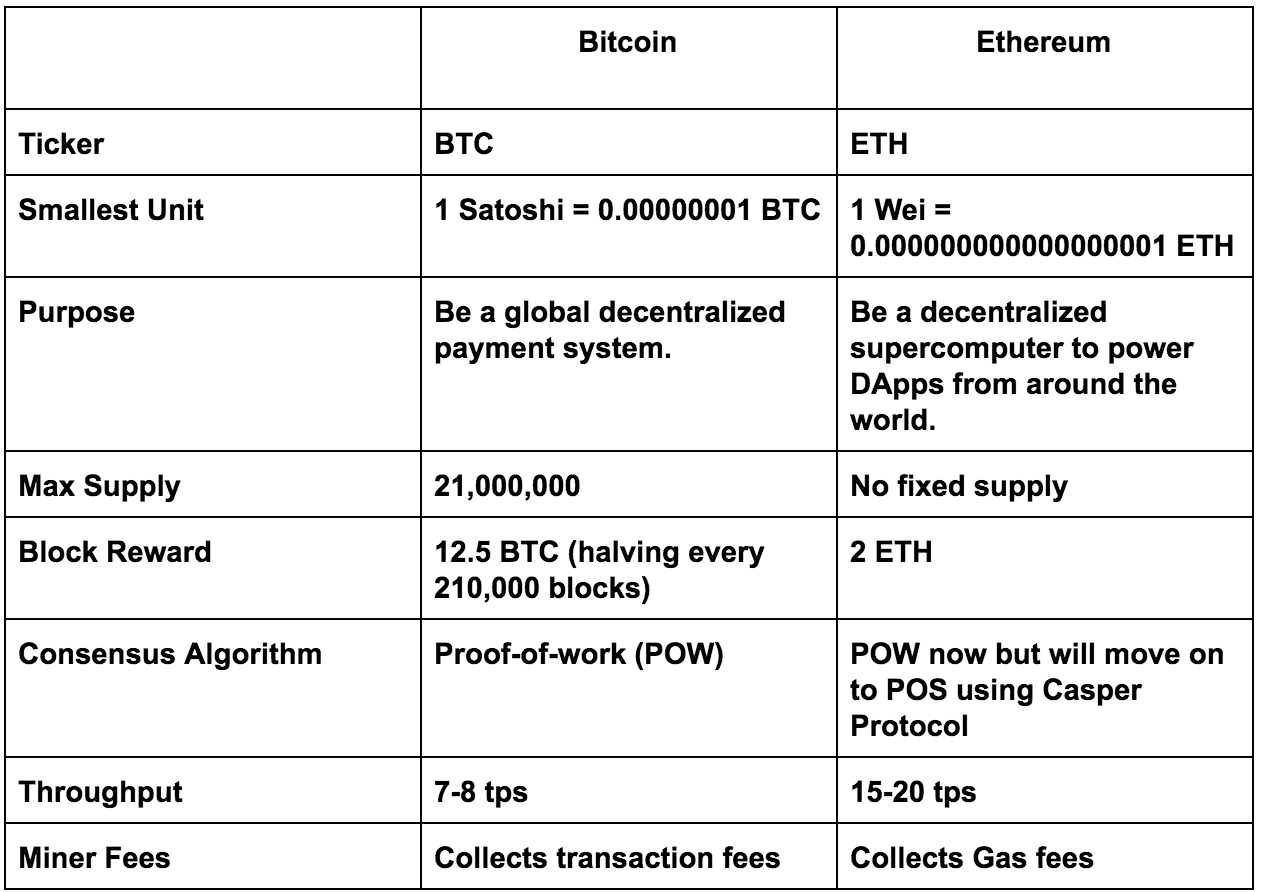
\includegraphics[scale=0.23]{comparison}
\end{frame}
%%%%%%%%%%%% Slide %%%%%%%%%%%%%%%%%%%%%%%%%%%%%%%%%%%%%%%%%%%%%%%%%%%
\begin{frame}
  \frametitle{Ethereum Accounts}
  User owns private keys to an account. \pause
  \begin{itemize}
  	\item \textcolor{brown}{Externally Owned Accounts:}
  	\begin{itemize}
		\item Owned by some external entity (person, corporation, etc.)
		\item Can send transactions to transfer  ether or trigger contract code.
		\item Contains: Address, Ether Balance.
	\end{itemize}
	\pause
	\item \textcolor{brown}{Contract Accounts:}
	\begin{itemize}
		\item ``Owned'' by contract.
		\item Code execution triggered by  transactions or function calls (msg).
		\item Contains: Address, Associated contract code, Persistent storage.
	\end{itemize}
  \end{itemize}
\end{frame}
%%%%%%%%%%%% Slide %%%%%%%%%%%%%%%%%%%%%%%%%%%%%%%%%%%%%%%%%%%%%%%%%%%
\begin{frame}
  \frametitle{Ethereum Smart Contracts Purposes}
  \pause
 	\begin{itemize}
 		\item Store and maintain data.
 		\begin{itemize}
			\item Data represents something useful to users or other contracts.
			\item Ex: a token currency or organization's membership.
		\end{itemize}
		\pause
		\item Manage contract or relationship between untrusting users.
		\begin{itemize}
			\item Ex: financial contracts, insurance.
		\end{itemize} \pause
		\item Provide functions to other contracts.
		\begin{itemize}
			\item Serving as a software library.
		\end{itemize}
		\item Complex Authentication.
 	\end{itemize}
\end{frame}
%%%%%%%%%%%% Slide %%%%%%%%%%%%%%%%%%%%%%%%%%%%%%%%%%%%%%%%%%%%%%%%%%%
\begin{frame}
  \frametitle{Ethereum Mining}
 	\begin{enumerate}
 		\item Download the entire Ethereum blockchain.
		\item Verify incoming transactions and Run Smart Contract code invoked by transactions.
		\item Create a block. 
		\item Find a valid nonce. 
		\item Broadcast your block. 
		\item Profit!
 	\end{enumerate}
\end{frame}
%%%%%%%%%%%% Slide %%%%%%%%%%%%%%%%%%%%%%%%%%%%%%%%%%%%%%%%%%%%%%%%%%%
\begin{frame}
  \frametitle{Ethereum Mining}
  	\begin{itemize}
  		\item Ref: \url{https://ethereum.org/en/whitepaper/}
  	\end{itemize}
 	\centering
	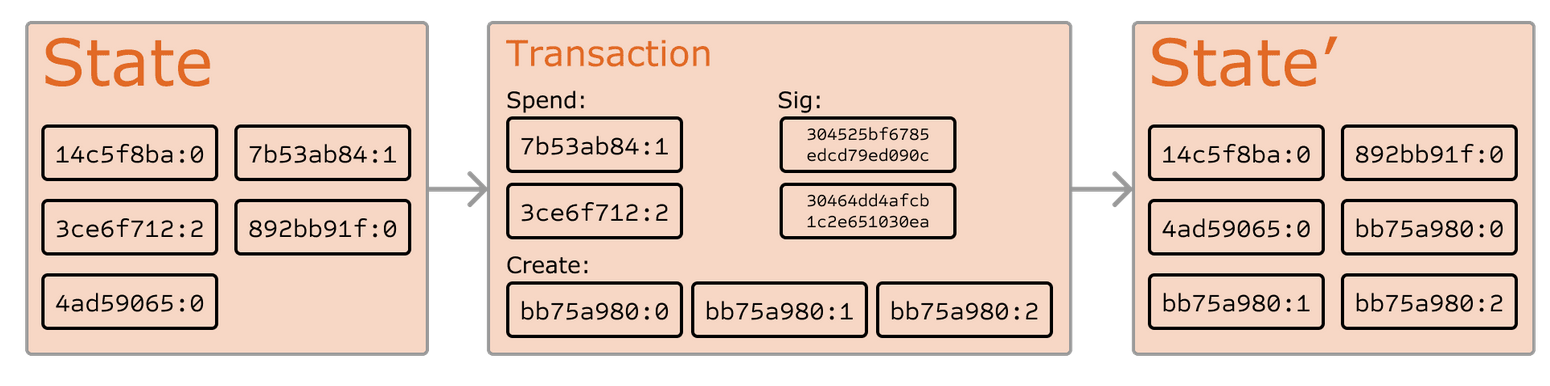
\includegraphics[scale=0.45]{states}
\end{frame}
%%%%%%%%%%%% Slide %%%%%%%%%%%%%%%%%%%%%%%%%%%%%%%%%%%%%%%%%%%%%%%%%%%
\begin{frame}
  \frametitle{Altcoins}
 	\centering
 	Ref: \url{https://coin360.com/}
	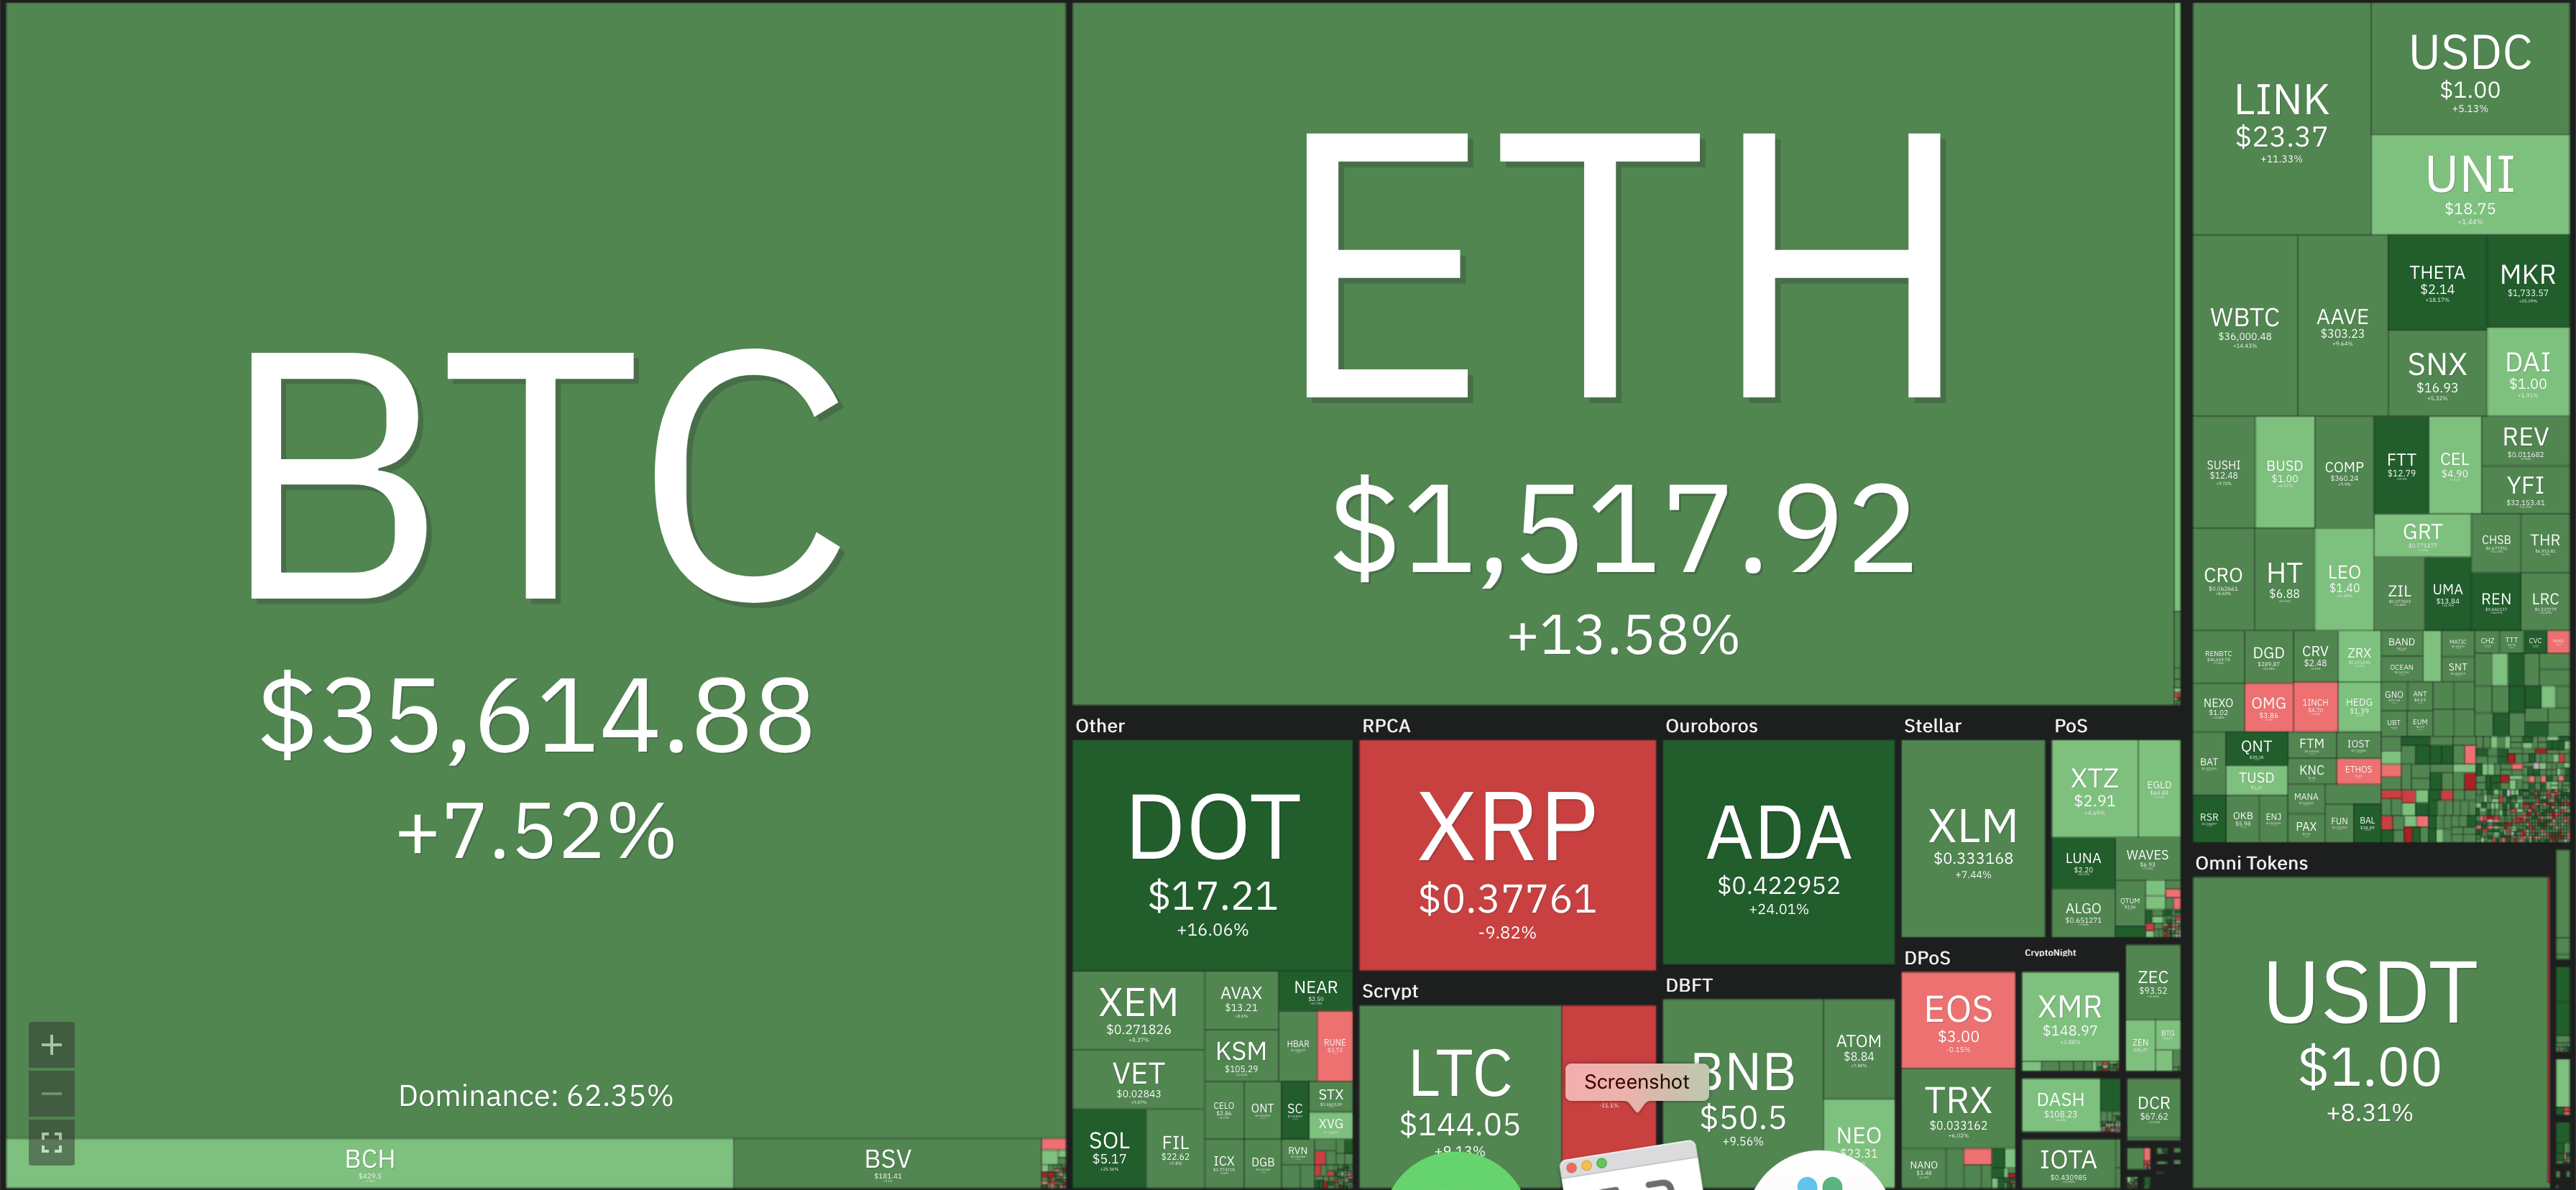
\includegraphics[scale=0.19]{altcoins}
\end{frame}
%%%%%%%%%%%% Slide %%%%%%%%%%%%%%%%%%%%%%%%%%%%%%%%%%%%%%%%%%%%%%%%%%%
\begin{frame}
  \frametitle{Features of altcoins}
  
	\begin{itemize}
		\item Better (or different) security.
			\begin{itemize}
				\item Mining puzzle.
			\end{itemize}
			\pause
		\item Contract/platform features. \pause
		\item Different parameters and monetary policy: inflation, inter block time. \pause
		\item Community or common interest support
	\end{itemize}
\end{frame}
%%%%%%%%%%%% Slide %%%%%%%%%%%%%%%%%%%%%%%%%%%%%%%%%%%%%%%%%%%%%%%%%%%
\begin{frame}
  \frametitle{Litecoin}
  \url{https://litecoin.org/}
  	\begin{itemize}
  		\item Litecoin launched in September 2011.
		\item Memory-hard mining puzzle.
  	\end{itemize}
  	
 	\centering
	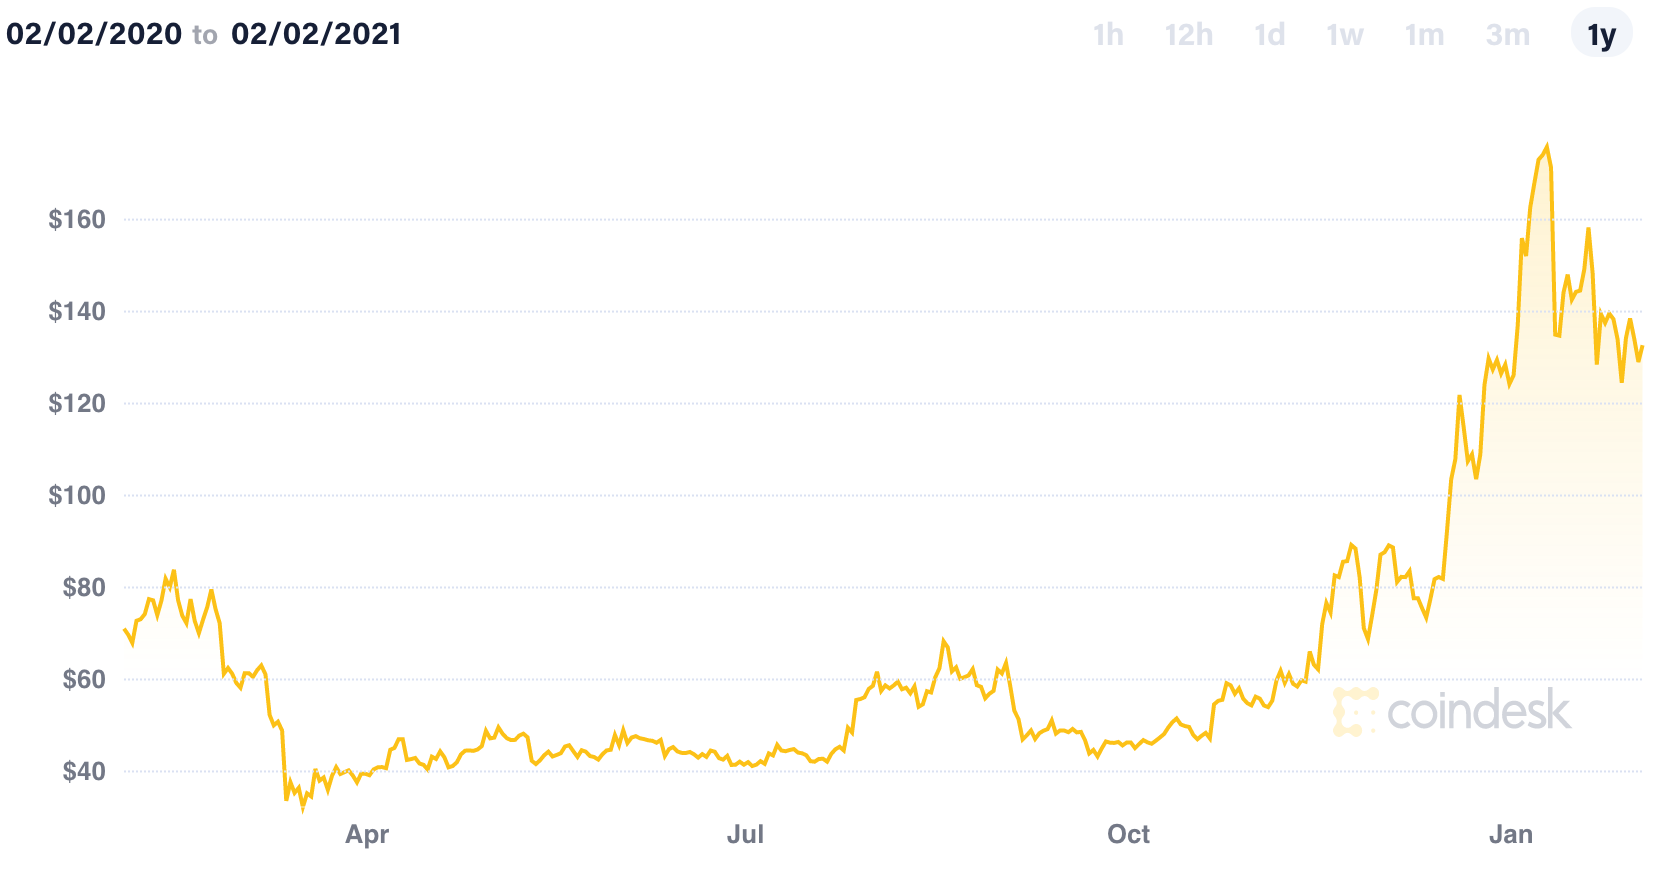
\includegraphics[scale=0.35]{litecoin}
\end{frame}

%%%%%%%%%%%% Slide %%%%%%%%%%%%%%%%%%%%%%%%%%%%%%%%%%%%%%%%%%%%%%%%%%%
\begin{frame}
  \frametitle{Dogecoin}
  \url{https://dogecoin.com/}
\begin{itemize}
	\item Launched in December 2013.
	\item Culture - tipping, charity, sponsorship.
\end{itemize}
 	\centering
	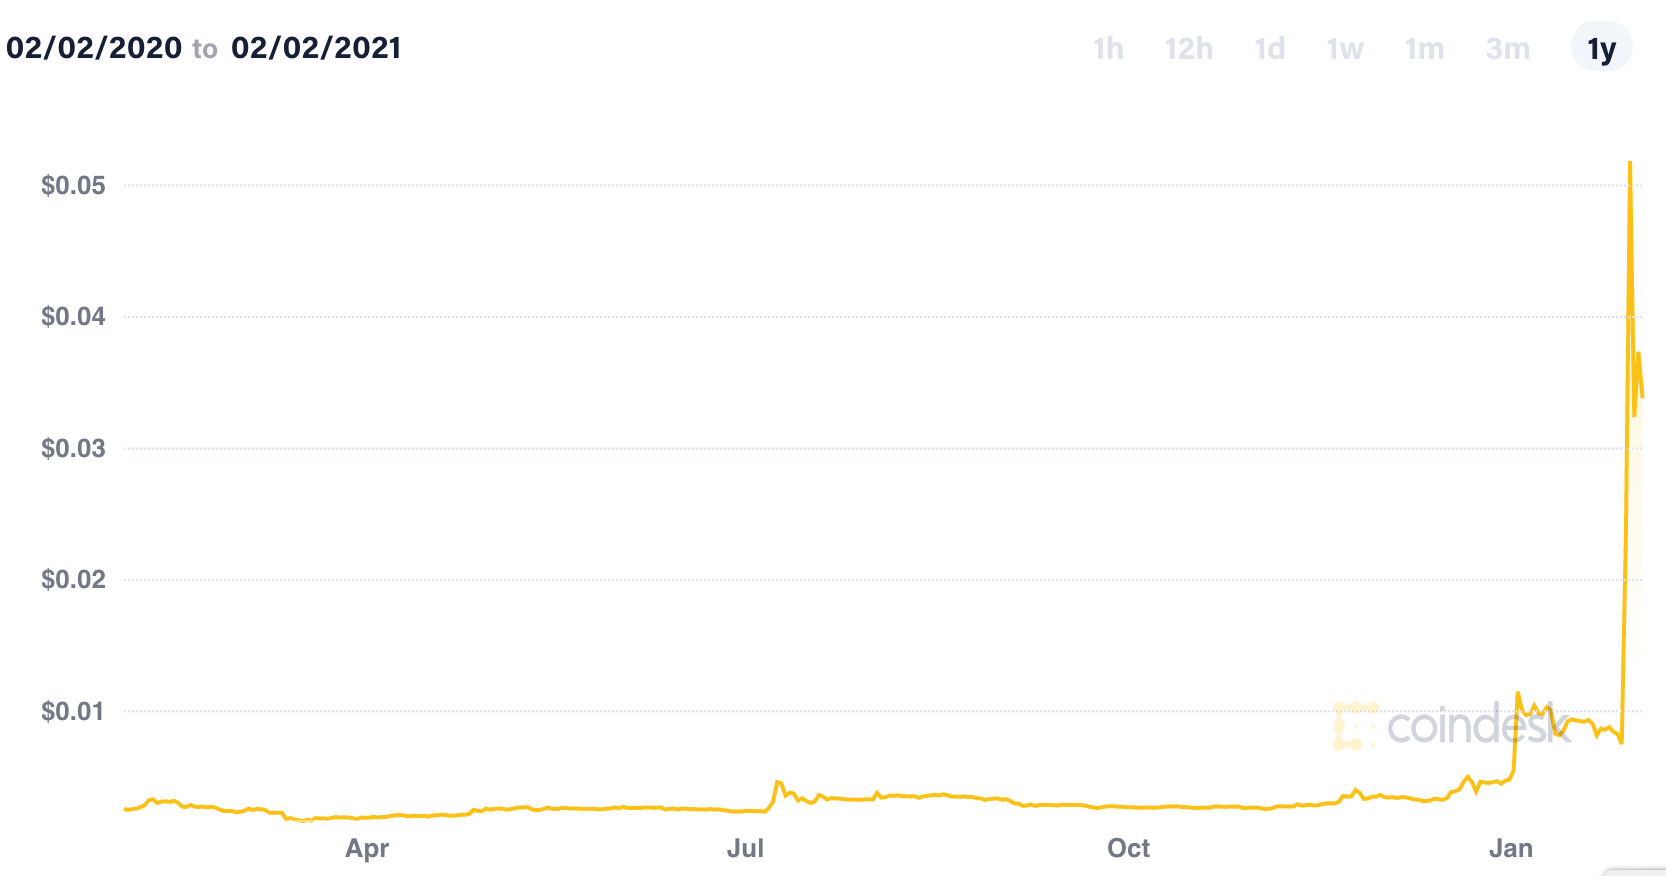
\includegraphics[scale=0.35]{dogecoin}
\end{frame}
%%%%%%%%%%%% Slide %%%%%%%%%%%%%%%%%%%%%%%%%%%%%%%%%%%%%%%%%%%%%%%%%%%
\begin{frame}
  \frametitle{Explore Alcoins}
  \url{https://www.coingecko.com}
\begin{itemize}
	\item Select one Altcoin.
	\pause
	\begin{itemize}
		\item When and why was it created?
		\item What are its features?
		\item What is its current status?
	\end{itemize}
\end{itemize}
\end{frame}

%%%%%%%%%%%% Slide %%%%%%%%%%%%%%%%%%%%%%%%%%%%%%%%%%%%%%%%%%%%%%%%%%%
\end{document}
